\scanpage{118}
% ms. line 01
Supposons maintenant que $(r_{\unsure{\nu|v}})$ soit la suite des
% ms. line 02
modules des zéros d'une fonction entière $f(z)$.
% ms. line 03
On aura $\displaystyle 2\pi n(r)=\int_0^{\deleted{\unsure{a}}2\pi}\frac{f'(re^{i\varphi})}{f(re^{i\varphi})}re^{i\varphi}\,d\varphi$, d'où
% ms. line 04
\[ \begin{aligned} 2\pi\int_a^b n(r)\mu(r)\,dr
&=\int_a^b\int_0^{2\pi}\frac{f'(re^{i\varphi})}{f(re^{i\varphi})}e^{i\varphi}\cdot\deleted{d\varphi}\ r\mu(r)\,dr\,d\varphi\\
% ms. line 05
&=\int_0^{2\pi}d\varphi\int_a^b\underbrace{\frac{f'(re^{i\varphi})}{f(re^{i\varphi})}e^{i\varphi}\,dr}_{d_r\log f(re^{i\varphi})}\ (r\mu(r)) \end{aligned} \]
% ms. line 06
\[ \int_a^b=\left[r\mu(r)\log f(re^{i\varphi})\right]_a^b-\int_a^b\log f(re^{i\varphi})\,d(r\mu(r)) \]
% ms. line 07
(en supposant $\mu(r)$ continûment différentiable)

% ms. line 08
-- On choisit brutalement la détermination
% ms. line 09
principale du logarithme -- pas de trouble,
% ms. line 10
car les intégrales \deleted{\unsure{si elles ont|simplement}} doubles
% ms. line 11
qui interviennent sont convergentes)
\figure{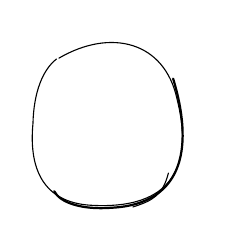
\begin{tikzpicture}[x=1cm,y=1cm,line cap=round]
\draw (.23,1.81) .. controls (.88,2.19) and (1.57,2.03) .. (1.73,1.29) .. controls (1.98,.29) and (1.52,-.10) .. (.67,-.06) .. controls (.08,-.04) and (-.16,.34) .. (-.10,.98) .. controls (-.09,1.37) and (.02,1.66) .. (.20,1.80);
\draw[thick] (1.68,1.55) .. controls (1.93,.73) and (1.85,-.04) .. (.90,-.09) .. controls (.51,-.12) and (.24,-.02) .. (.17,.12);
\draw (1.62,.35) .. controls (1.55,.07) and (1.42,.00) .. (1.17,-.08);
\end{tikzpicture}}
% ms. line 12
D'où, en substituant, intervertissant les signes $\int\!\int$, et
% slanted
% ms. line 12a
\margin{en prenant les parties réelles}
% ms. line 13
\[ \boxed{\displaystyle \deleted{2\pi}\int_{\unsure{a}}^b n(r)\mu(r)\,dr=\left[r\mu(r)V(r)\right]_a^b-\int_a^b V(r)\,d(r\mu(r))} \]
% ms. line 14
où \qquad \uline{$\displaystyle V(r)=\frac1{2\pi}\int_0^{2\pi}\log|f(re^{i\varphi})|\,d\varphi$}
% ms. line 15
Prenons $\mu(r)=-\lambda'(r)$, on obtient \enspace $(0<a<b<+\infty$
% ms. line 16
\[ \boxed{\begin{aligned}\sum_{\substack{\nu\\a<r_\nu<b}}\lambda(r_\nu)^{\deleted{\unsure{\alpha}}}&=\lambda(b)n(b-0)-\lambda(a)n(a+0)+[r\mu(r)V(r)]_a^b\deleted{\unsure{+\int V(r)\,d(r\mu)|+\int}}\\
% ms. line 17
&\qquad+\int_a^b V(r)\,d(r\lambda'(r))\end{aligned}} \]
% archive sheet number: 119
